\chapter{Indoor spatio-temporal movement patterns}
\section{Introduction}
As described in the firs part of this report, Wi-Fi tracking data can be used to
identify movement between buildings. Given that indoor areas are usually better
covered with Wi-Fi access points than outdoor areas, it is natural to also look
at movement inside buildings. The following section describes our method of
identifying and visualizing indoor movement in the Faculty of Architecture of TU
Delft.

The process of indoor movement analysis is conducted along the steps below,
thus the section also follows this structure:

\begin{enumerate}
    \item Delineate building parts based on the layout of access points
and the division of the building (e.g. department, canteen, building wing), and
group the access point into building parts.
    \item Identify movements in the data between building parts.
    \item Create a route network that connects the building parts and
    is constrained on the corridors of the building.
    \item Assign the movements to the route network.
    \item Visualize the movement along the indoor network.
\end{enumerate}

\section{Theory / methods}
After identifying movement between different buildings, the next level is to do
so between different parts inside a building. These parts represent
functional or spatial divisions inside a building, e.g. departments, community
areas, building wings and are referred to as \textit{building part}.

A prerequisite of the method is to know the at least room level location of the
access points in the respective building. At the time when the project
was carried out, the detailed access point locations were availably only for the
Faculty of Architecture. Thus the focus on this particular building.

As opposed to outdoor pedestrian movement which is not necessarily constrained
on a fixed network, indoor movement is constrained by the layout of the
respective building. The building parts of the Faculty of Architecture can be
represented by its underlying graph, having the building parts as nodes and the
corridors as edges \autoref{figure:bk_graph}. Then indoor movement is
necessarily constrained on this underlying graph.

\begin{figure}[H]
\centering
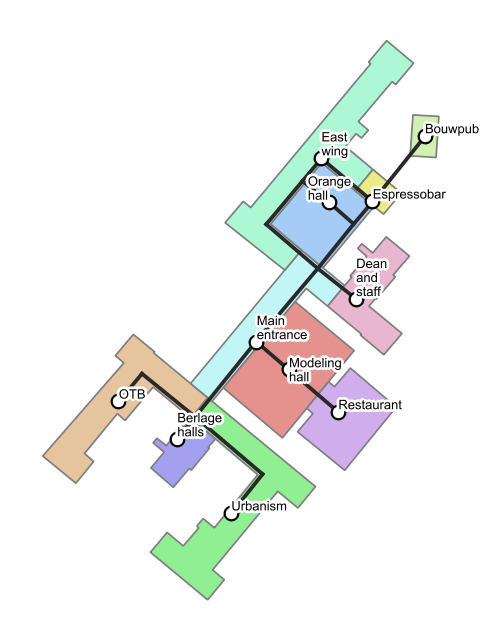
\includegraphics[scale=0.8]{bk_BG_bparts.png}
\captionsetup{justification=centering}
\caption{Building parts on the ground floor of the Faculty of Architecture and
its underlying graph.}
\label{figure:bk_graph}
\end{figure}

The Wi-Fi system of the TU Delft campus has a five minute scan interval, which
is too coarse to catch detailed movement indoor. As five minutes is
sufficient to reach any two locations in the building taking any route.
Therefore not the movement trajectory itself is identified from the data, but
the fact of relocation from origin to destination. Then the path of the movement
can also be identified by analysing the layout of the building. For example if a
person stayed at the Restaurant, then soon after he stayed at the Orange hall,
he necessarily had to traverse the corridors in-between these two locations. Our
method is based on this assumption.

Due to the building layout, in most of the cases there is only one possible
direct route between two building parts. However, in case of multiple route
options, the exact route of a movement is assumed to be the shortest route 
between origin and
destination.

\section{Implementation}
Balázs: describing how the map visualization works and implemented, writing in 
a separate document

\section{Results}

